\documentclass{beamer}
\usepackage[utf8]{inputenc}
\usepackage{graphicx, epsfig}
\usepackage{amsmath,mathrsfs,amsfonts,amssymb}
\usepackage{floatflt}
\usepackage{epic,ecltree}
\usepackage{mathtext}
\usepackage{fancybox}
\usepackage{fancyhdr}
\usepackage{multirow}
\usepackage{enumerate}
\usepackage{epstopdf}
\usepackage{multicol}
\usepackage{algorithm}
\usepackage[noend]{algorithmic}
\usepackage{tikz}
\usepackage{blindtext}
\usetheme{default}%{Singapore}%{Warsaw}%{Warsaw}%{Darmstadt}
\usecolortheme{default}

\setbeamerfont{title}{size=\Huge}
\setbeamertemplate{footline}[page number]{}

\setbeamertemplate{section in toc}[sections numbered]


\makeatletter
\newcommand\HUGE{\@setfontsize\Huge{35}{40}}
\makeatother    

\setbeamerfont{title}{size=\HUGE}
\beamertemplatenavigationsymbolsempty

% latin bold lower
\newcommand{\ba}{\mathbf{a}} 
\newcommand{\bc}{\mathbf{c}} 
\newcommand{\be}{\mathbf{e}} 
\newcommand{\bh}{\mathbf{h}} 
\newcommand{\bp}{\mathbf{p}} 
\newcommand{\bt}{\mathbf{t}} 
\newcommand{\bs}{\mathbf{s}} 
\newcommand{\bu}{\mathbf{u}} 
\newcommand{\bv}{\mathbf{v}} 
\newcommand{\bw}{\mathbf{w}} 
\newcommand{\bx}{\mathbf{x}} 
\newcommand{\by}{\mathbf{y}} 
\newcommand{\bz}{\mathbf{z}} 

% latin bold upper
\newcommand{\bA}{\mathbf{A}} 
\newcommand{\bB}{\mathbf{B}} 
\newcommand{\bC}{\mathbf{C}} 
\newcommand{\bI}{\mathbf{I}} 
\newcommand{\bJ}{\mathbf{J}} 
\newcommand{\bL}{\mathbf{L}} 
\newcommand{\bM}{\mathbf{M}} 
\newcommand{\bP}{\mathbf{P}}
\newcommand{\bQ}{\mathbf{Q}} 
\newcommand{\bR}{\mathbf{R}} 
\newcommand{\bT}{\mathbf{T}} 
\newcommand{\bU}{\mathbf{U}} 
\newcommand{\bV}{\mathbf{V}} 
\newcommand{\bW}{\mathbf{W}} 
\newcommand{\bX}{\mathbf{X}} 
\newcommand{\bY}{\mathbf{Y}} 
\newcommand{\bZ}{\mathbf{Z}} 

% latin cal upper
\newcommand{\cF}{\mathcal{F}} 
\newcommand{\cG}{\mathcal{G}} 
\newcommand{\cI}{\mathcal{I}} 
\newcommand{\cL}{\mathcal{L}} 
\newcommand{\cM}{\mathcal{M}} 
\newcommand{\cN}{\mathcal{N}} 
\newcommand{\cS}{\mathcal{S}} 
\newcommand{\cT}{\mathcal{T}} 
\newcommand{\cW}{\mathcal{W}} 
\newcommand{\cX}{\mathcal{X}} 
\newcommand{\cZ}{\mathcal{Z}} 

% latin bb upper
\newcommand{\bbE}{\mathbb{E}} 
\newcommand{\bbI}{\mathbb{I}} 
\newcommand{\bbP}{\mathbb{P}} 
\newcommand{\bbR}{\mathbb{R}} 

% greek bold lower
\newcommand{\bepsilon}{\boldsymbol{\epsilon}} 
\newcommand{\btheta}{\boldsymbol{\theta}} 
\newcommand{\blambda}{\boldsymbol{\lambda}} 
\newcommand{\bpi}{\boldsymbol{\pi}} 
\newcommand{\bmu}{\boldsymbol{\mu}} 
\newcommand{\bsigma}{\boldsymbol{\sigma}} 
\newcommand{\bphi}{\boldsymbol{\phi}} 

% greek bold upper
\newcommand{\bSigma}{\boldsymbol{\Sigma}} 

\DeclareMathOperator*{\argmin}{arg\,min}
\DeclareMathOperator*{\argmax}{arg\,max}

\newcommand{\createdgmtitle}[1]{\title[\hbox to 56mm{Deep Generative Models  \hfill\insertframenumber\,/\,\inserttotalframenumber}]
	{\vspace{1cm} \\ Deep Generative Models \\ {\Huge Lecture #1}}
	\author{Roman Isachenko}
	\institute{
	Moscow Institute of Physics and Technology
	} 
	\date{2023, Autumn}
}

\usepackage{tikz}
\usetikzlibrary{arrows,shapes,positioning,shadows,trees}

\newcommand\myfootnote[1]{%
  \tikz[remember picture,overlay]
  \draw (current page.south west) +(1in + \oddsidemargin,0.5em)
  node[anchor=south west,inner sep=0pt]{\parbox{\textwidth}{%
      \rlap{\rule{10em}{0.4pt}}\raggedright\scriptsize \textit{#1}}};}

\newcommand\myfootnotewithlink[2]{%
  \tikz[remember picture,overlay]
  \draw (current page.south west) +(1in + \oddsidemargin,0.5em)
  node[anchor=south west,inner sep=0pt]{\parbox{\textwidth}{%
      \rlap{\rule{10em}{0.4pt}}\raggedright\scriptsize\href{#1}{\textit{#2}}}};}
      
\AtBeginSection[]
      {
      	\begin{frame}{Outline}
      		\tableofcontents[currentsection]
      	\end{frame}
      }
      \AtBeginSubsection[]{
      	\begin{frame}{Outline}
      		\tableofcontents[currentsection,currentsubsection]
      	\end{frame}
}
\createdgmtitle{11}
%--------------------------------------------------------------------------------
\begin{document}
%--------------------------------------------------------------------------------
\begin{frame}[noframenumbering,plain]
%\thispagestyle{empty}
\titlepage
\end{frame}
%=======
\begin{frame}{Recap of previous lecture}
	Let take some pretrained image classification model to get the conditional label distribution $p(y | \bx)$ (e.g. ImageNet classifier).
	\begin{block}{Evaluation of likelihood-free models}
		\begin{itemize}
			\item Sharpness $\Rightarrow$ low $H(y | \bx) = - \sum_{y} \int_{\bx} p(y, \bx) \log p(y | \bx) d\bx$.
			\item Diversity $\Rightarrow$ high $H(y)  = - \sum_{y} p(y) \log p(y)$.
		\end{itemize}
	\end{block}
	\vspace{-0.3cm}
	\begin{block}{Inception Score}
		\vspace{-0.2cm}
		\[
			IS = \exp(H(y) - H(y | \bx)) = \exp \left( \bbE_{\bx} KL(p(y | \bx) || p(y)) \right)
		\]
		\vspace{-0.5cm}
	\end{block}
	\begin{block}{Frechet Inception Distance}
		\vspace{-0.3cm}
		\[
			D^2 (\pi, p) = \| \mathbf{m}_{\pi} - \mathbf{m}_{p}\|_2^2 + \text{Tr} \left( \bSigma_{\pi} + \bSigma_p - 2 \sqrt{\bSigma_{\pi} \bSigma_p} \right).
		\]
		\vspace{-0.5cm}
	\end{block}
	FID is related to moment matching.
	
	\myfootnote{\href{https://arxiv.org/abs/1606.03498}{Salimans T. et al. Improved Techniques for Training GANs, 2016} \\
	\href{https://arxiv.org/abs/1706.08500}{Heusel M. et al. GANs Trained by a Two Time-Scale Update Rule Converge to a Local Nash Equilibrium, 2017} }
\end{frame}
%=======
\begin{frame}{Recap of previous lecture}
		\begin{itemize}
			\item $\cS_{\pi} = \{\bx_i\}_{i=1}^{n} \sim \pi(\bx)$ -- real samples;
			\item $\cS_{p} = \{\bx_i\}_{i=1}^{n} \sim p(\bx | \btheta)$ -- generated samples.
		\end{itemize}
		Embed samples using pretrained classifier network (as previously):
		\[
			\cG_{\pi} = \{\mathbf{g}_i\}_{i=1}^n, \quad \cG_{p} = \{\mathbf{g}_i\}_{i=1}^n.
		\]
		Define binary function:
		\[
			f(\mathbf{g}, \cG) = 
			\begin{cases}
				1, \text{if exists } \mathbf{g}' \in \cG: \| \mathbf{g}  - \mathbf{g}'\|_2 \leq \| \mathbf{g}' - \text{NN}_k(\mathbf{g}', \cG)\|_2; \\
				0, \text{otherwise.}
			\end{cases}
		\]
		\[
			\text{Precision} (\cG_{\pi}, \cG_{p}) = \frac{1}{n} \sum_{\mathbf{g} \in \cG_{p}} f(\mathbf{g}, \cG_{\pi}); \quad \text{Recall} (\cG_{\pi}, \cG_{p}) = \frac{1}{n} \sum_{\mathbf{g} \in \cG_{\pi}} f(\mathbf{g}, \cG_{p}).
		\]
		\vspace{-0.4cm}
		\begin{figure}
			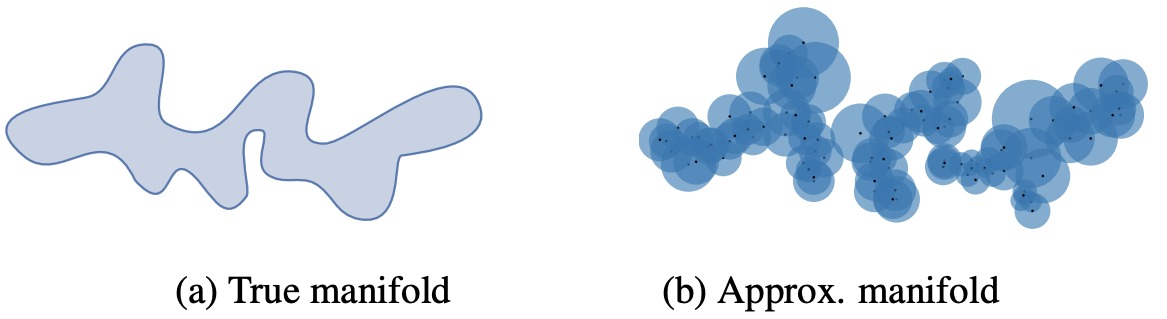
\includegraphics[width=0.7\linewidth]{figs/pr_k_nearest}
		\end{figure}
		\myfootnotewithlink{https://arxiv.org/abs/1904.06991}{Kynkäänniemi T. et al. Improved precision and recall metric for assessing generative models, 2019}
\end{frame}
%=======
\begin{frame}{Recap of previous lecture}
	\begin{block}{Discrete VAE latents}
		\begin{itemize}
			\item Define dictionary (word book) space $\{\be_k\}_{k=1}^K$, where $\be_k \in \bbR^C$, $K$ is the size of the dictionary.
			\item Our variational posterior $q(c | \bx, \bphi) = \text{Categorical}(\bpi(\bx, \bphi))$ (encoder) outputs discrete probabilities vector.
			\item We sample $c^*$ from $q(c | \bx, \bphi)$ (reparametrization trick analogue).
			\item Our generative distribution $p(\bx | \be_{c^*}, \btheta)$ (decoder).
		\end{itemize}
	\end{block}
	\vspace{-0.3cm}
	\begin{block}{ELBO}
		\vspace{-0.7cm}
		\[
		\mathcal{L} (\bphi, \btheta)  = \mathbb{E}_{q(c | \bx, \bphi)} \log p(\bx | c, \btheta) - KL(q(c| \bx, \bphi) || p(c)) \rightarrow \max_{\bphi, \btheta}.
		\]
		\vspace{-0.7cm}
	\end{block}
	\begin{block}{KL term}
		\vspace{-0.4cm}
		\[
		KL(q(c| \bx, \bphi) || p(c)) = - H(q(c | \bx, \bphi)) + \log K. 
		\]
	\end{block}
	Is it possible to make reparametrization trick? (we sample from discrete distribution now!).
\end{frame}
%=======
\begin{frame}{Outline}
	\tableofcontents
\end{frame}
%=======
\section{Neural ODE}
%=======
\begin{frame}{Neural ODE}
	Consider Ordinary Differential Equation (ODE)
	\begin{align*}
	    \frac{d \bz(t)}{dt} &= f(\bz(t), t, \btheta); \quad \text{with initial condition }\bz(t_0) = \bz_0. \\
	    \bz(t_1) &= \int^{t_1}_{t_0} f(\bz(t), t, \btheta) d t  + \bz_0 = \text{ODESolve}(\bz(t_0), f, t_0,t_1, \btheta).
	\end{align*}
	\vspace{-0.4cm}
	\begin{block}{Euler update step}
		\vspace{-0.6cm}
		\[
		    \frac{\bz(t + \Delta t) - \bz(t)}{\Delta t} = f(\bz(t), t, \btheta) \,\, \Rightarrow \,\, \bz(t + \Delta t) = \bz(t) + \Delta t \cdot f(\bz(t), t, \btheta)
		\]
		\vspace{-0.7cm}
	\end{block}
	\begin{block}{Residual block}
		\begin{minipage}[t]{0.7\columnwidth}
			\vspace{-0.4cm}
			\[
				\bz_{t + 1} = \bz_t + f(\bz_t, \btheta)
			\]
			\vspace{-0.6cm}
			\begin{itemize}
				 \item It is equavalent to Euler update step for solving ODE with $\Delta t = 1$!
				 \item Euler update step is unstable and trivial. There are more sophisticated methods.
			\end{itemize}
		\end{minipage}%
		\begin{minipage}[t]{0.3\columnwidth}
			\vspace{-0.2cm}
			\begin{figure}
			    \centering
			    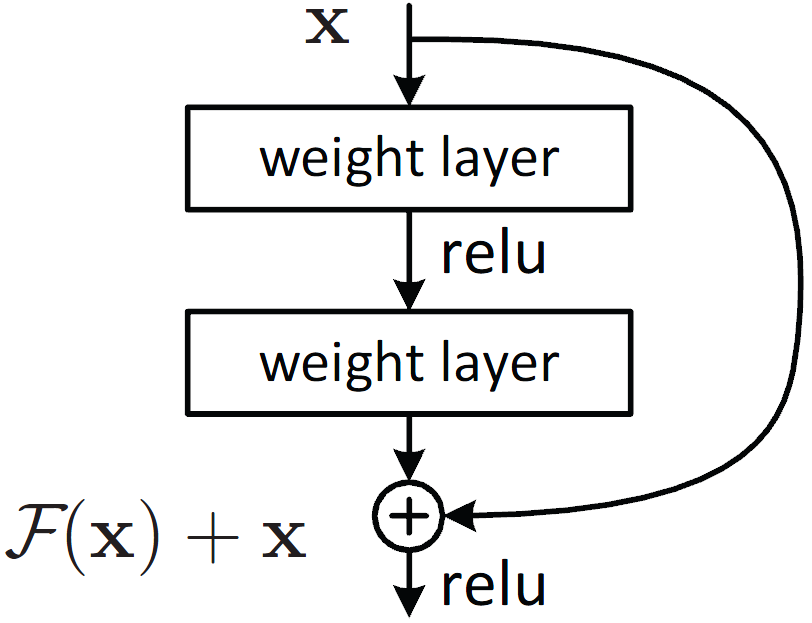
\includegraphics[width=\linewidth]{figs/resnet_1.png}
			\end{figure}
		\end{minipage}
		\vspace{-0.4cm}
	\end{block}

	\myfootnotewithlink{https://arxiv.org/abs/1806.07366}{Chen R. T. Q. et al. Neural Ordinary Differential Equations, 2018}   
\end{frame}
%=======
\begin{frame}{Neural ODE}
	\begin{block}{Residual block}
	\vspace{-0.4cm}
	\[
	    \bz_{t+1} = \bz_t + f(\bz_t, \btheta).
	\]
	\vspace{-0.4cm}
	\end{block}
	In the limit of adding more layers and taking smaller steps, we parameterize the continuous dynamics of hidden units using an ODE specified by a neural network: 
	\[
	    \frac{d \bz(t)}{dt} = f(\bz(t), t, \btheta); \quad \bz(t_0) = \bx; \quad \bz(t_1) = \by.
	\]
	\begin{minipage}[t]{0.4\columnwidth}
		\begin{figure}
			\centering
			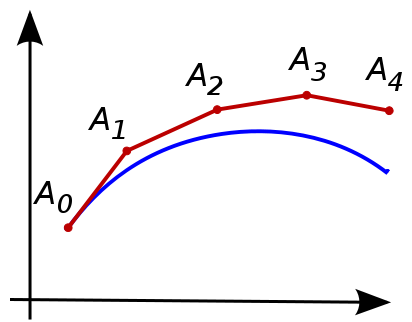
\includegraphics[width=0.8\linewidth]{figs/euler}
		\end{figure}
	\end{minipage}%
	\begin{minipage}[t]{0.6\columnwidth}
		\vspace{-0.4cm}
		\begin{figure}
			\centering
			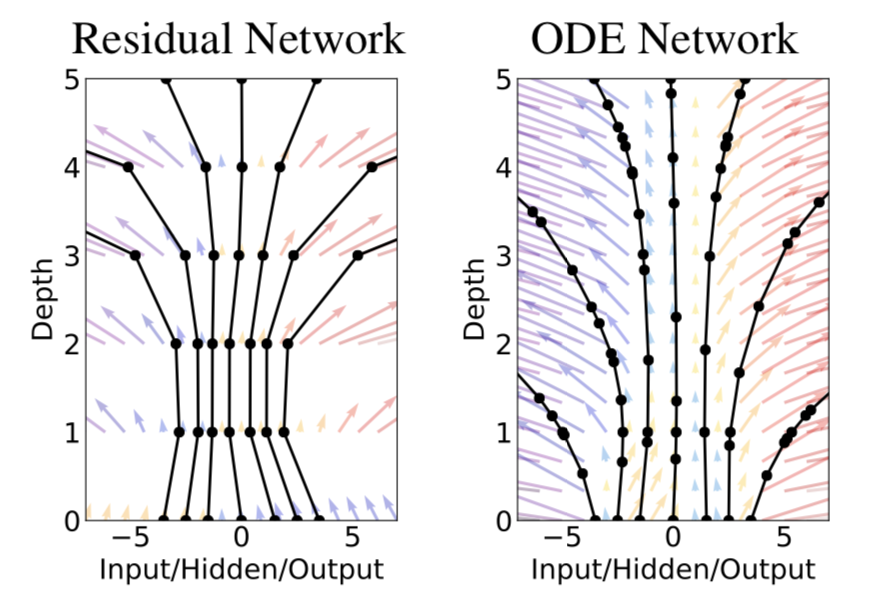
\includegraphics[width=0.9\linewidth]{figs/resnet_vs_neural_ode.png}
		\end{figure}
	\end{minipage}

	\myfootnotewithlink{https://arxiv.org/abs/1806.07366}{Chen R. T. Q. et al. Neural Ordinary Differential Equations, 2018}   
\end{frame}
%=======
\begin{frame}{Neural ODE}
	\begin{block}{Forward pass (loss function)}
		\vspace{-0.8cm}
		\begin{align*}
			L(\by) = L(\bz(t_1)) &= L\left( \bz(t_0) + \int_{t_0}^{t_1} f(\bz(t), t, \btheta) dt \right) \\ &= L\bigl(\text{ODESolve}(\bz(t_0), f, t_0,t_1, \btheta) \bigr)
		\end{align*}
	\vspace{-0.5cm}
	\end{block}
	\textbf{Note:} ODESolve could be any method (Euler step, Runge-Kutta methods).
	\begin{block}{Backward pass (gradients computation)}
		For fitting parameters we need gradients:
		\[
			\ba_{\bz}(t) = \frac{\partial L(\by)}{\partial \bz(t)}; \quad \ba_{\btheta}(t) = \frac{\partial L(\by)}{\partial \btheta(t)}.
		\]
		In theory of optimal control these functions called \textbf{adjoint} functions. 
		They show how the gradient of the loss depends on the hidden state~$\bz(t)$ and parameters $\btheta$.
	\end{block}

	\myfootnotewithlink{https://arxiv.org/abs/1806.07366}{Chen R. T. Q. et al. Neural Ordinary Differential Equations, 2018}     
\end{frame}
%=======
\begin{frame}{Summary}
	\begin{itemize}
		\item Residual networks could be interpreted as solution of ODE with Euler method.
	\end{itemize}
\end{frame}
%=======
\end{document} 